\FloatBarrier
\subsection{Question 2}
By cancelling out the zeros of system,  $A_o $ will be of degre  $0$. The refrence model will be calculated based on 
\autoref{code:str21} . The main difference in zero cancellation is the calculations required for determining $S$ and $R$ parameters. The system polynomials are estimated using RLS method. \autoref{fig:str11} shows the system output and control effort for indirect STR with zero cancellation.  \autoref{fig:str12} demonstrates the variation of parameter values over simulation time.

\begin{code}
	\begin{matlabcode}{firstnumber = 1}
%% Parameters
cancel = 1; % 0 no zero cancel, 1 all zero cancel
noise = 0; % if 1 white noise, 2 colored noise
distrubance = 1; % set to 1 for step disturbance
distrubance_fix = 0; % set to 1 to fix system
integral_fix = 0; % set 1 to limit u
vlimit = 4; % limit of u
lamda = 1;
. . .
if cancel
	sys_ref_dis = tf([0 sum(Am) 0],Am,Gz.Ts) ;
. . .
if cancel
	A0 = 0;
	Ac = poly([A0 roots(B)']) ;
. . .
if cancel
	S = zeros(1,numel(Am)-1);
	R = zeros(1,numel(Am)-1);
	R(1) = 1;
	for j = 1:numel(Am)-1
		S(j) = (Am(j+1)-Aes(j+1))/Bes(1);
	end
	for j = 2:3
		R(j) = Bes(j)/Bes(1);
	end
	T = [0,Bm(2)/Bes(1),0] ;
	\end{matlabcode}
	\captionof{listing}{Impelementation of Indirect STR with zero cancellation}
	\label{code:str21}
\end{code}

\begin{figure}
	\centering
	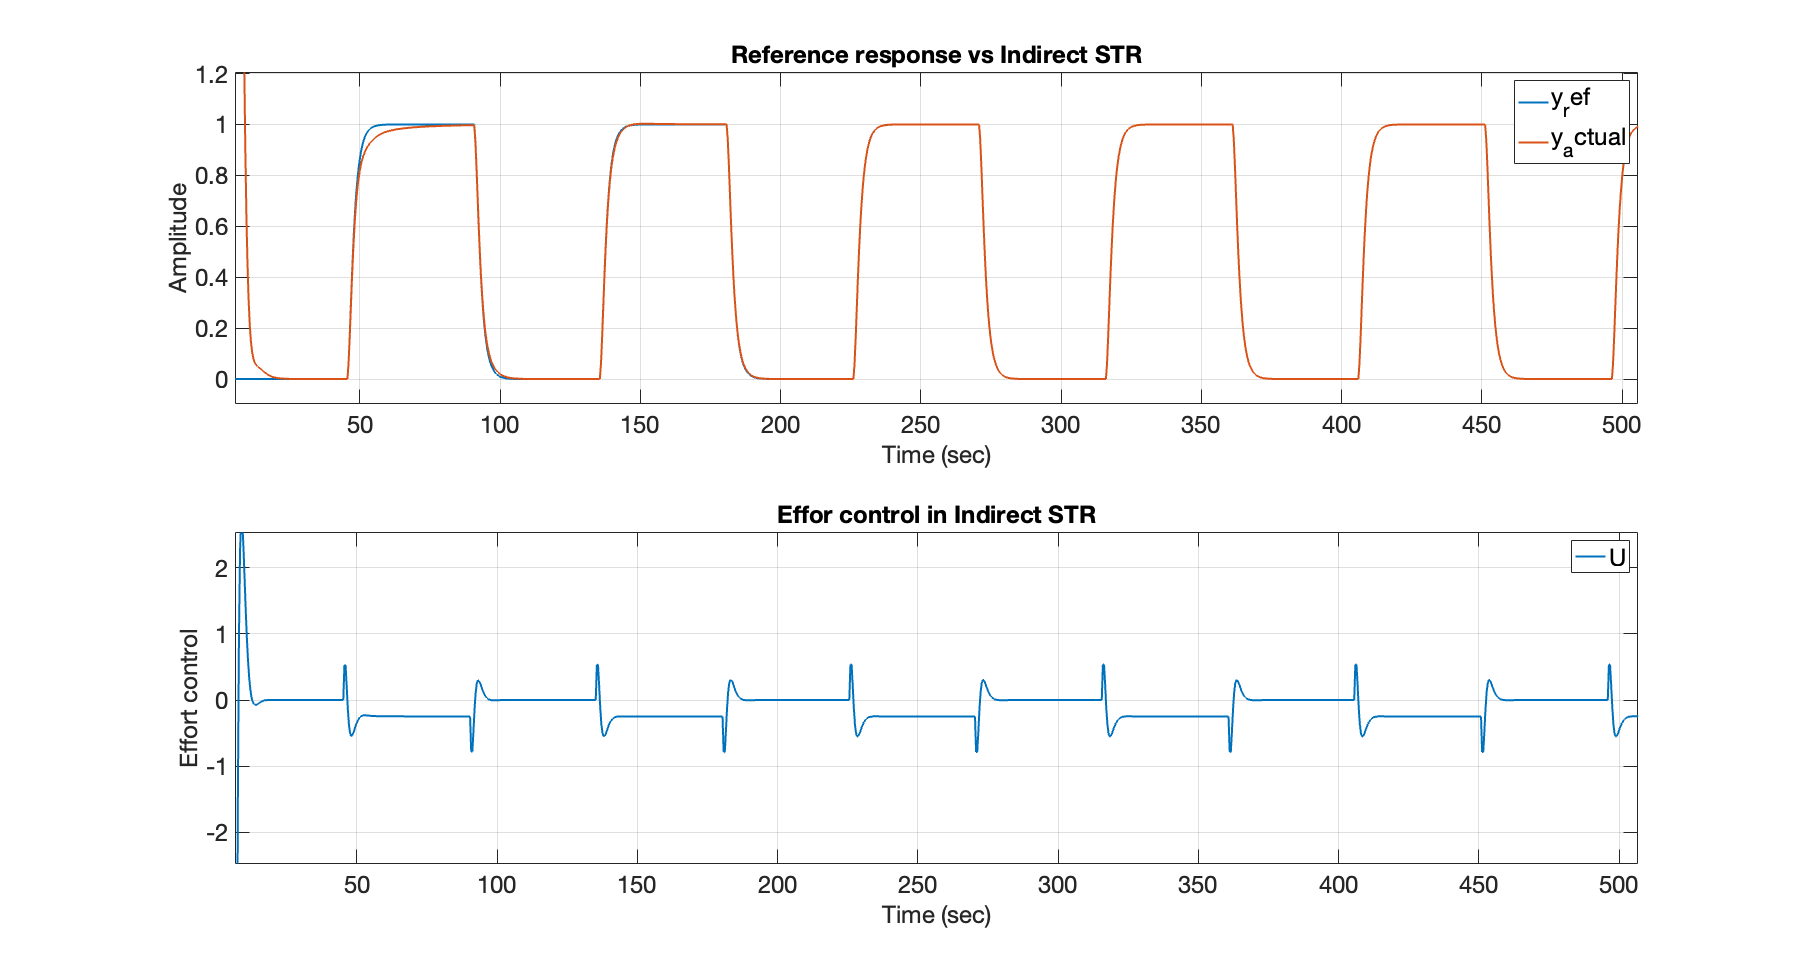
\includegraphics[width=\textwidth]{images/str21.png}
	\caption{Indirect STR ystem response with zero cancellation}
	\label{fig:str21}
\end{figure}

\begin{figure}
	\centering
	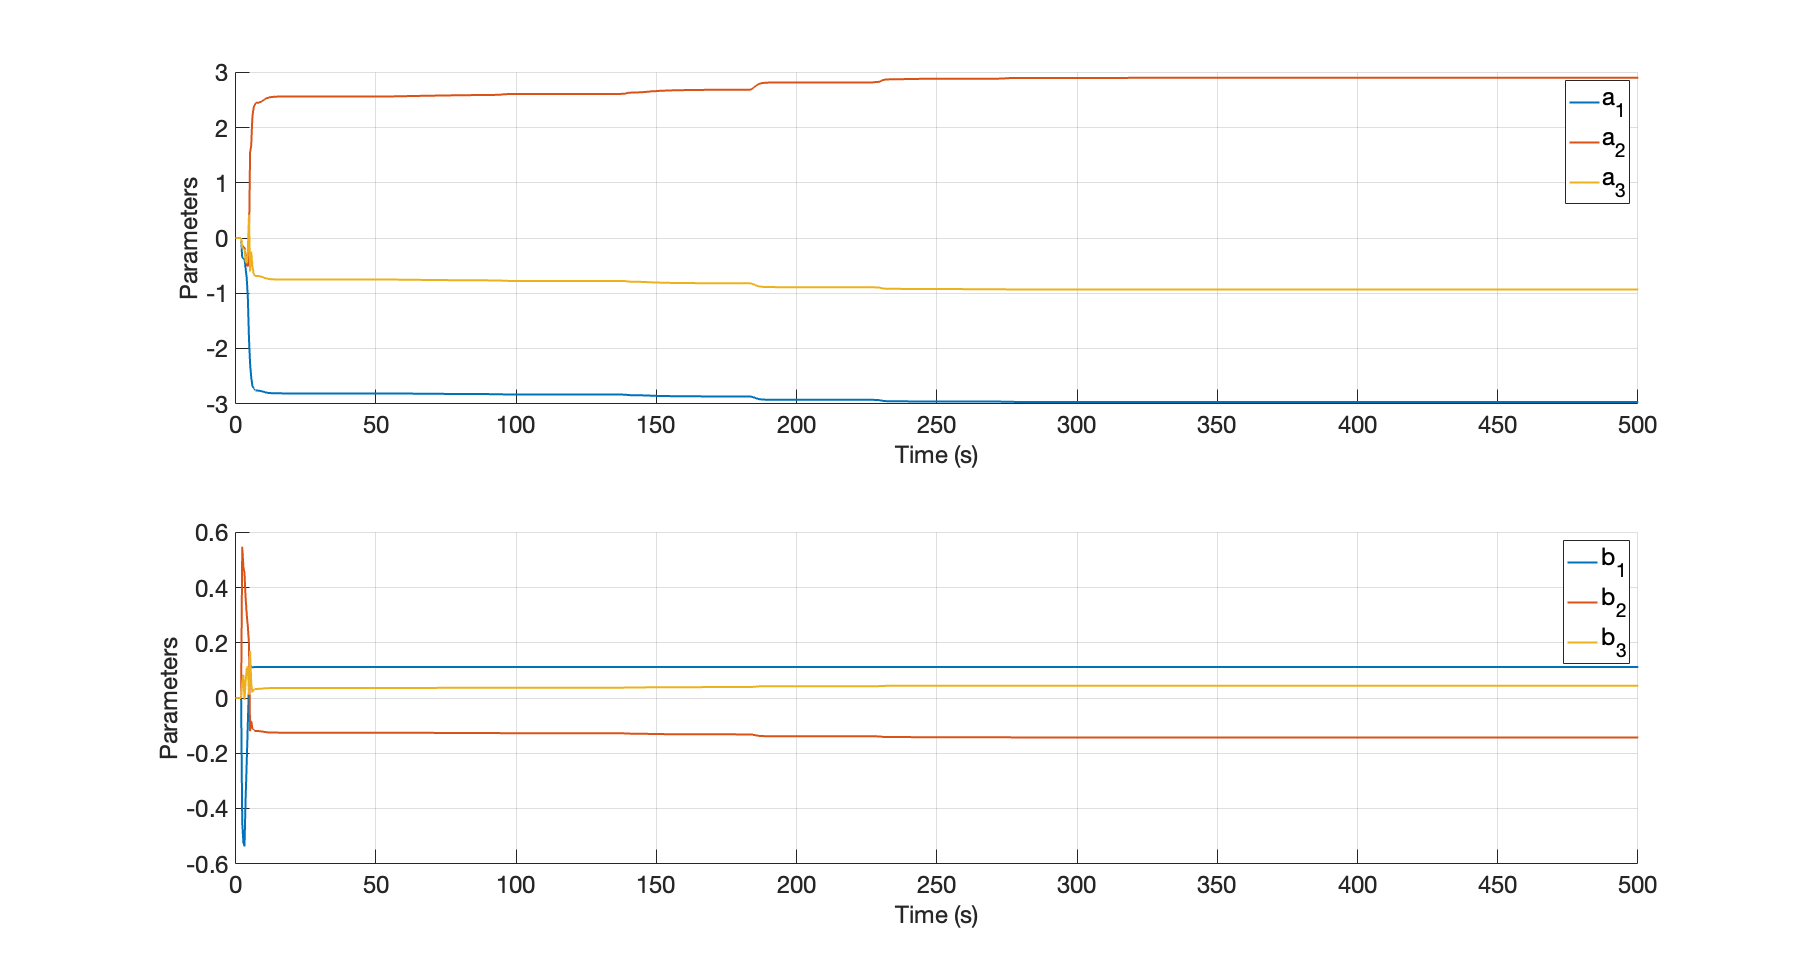
\includegraphics[width=\textwidth]{images/str22.png}
	\caption{System parameters in indirect STR with zero cancellation}
	\label{fig:str22}
\end{figure}

The code  for this section is available at \lstinline|assignment2/part2/STR1_indirect.m|. By changing the $change=0$ to $1$ system will calculate the $R$ and $S$ and determine other parameters required for Indirect STR with zero cancellation. The Diophantine equation solver code is at \lstinline|assignment2/part2/Diophantine.m| and RLS impelementation is located at \lstinline|assignment2/part2/RLS.m|.
